% !TeX program = xelatex

\documentclass[a4paper,10pt]{article}
\usepackage{marvosym}
\usepackage{fontspec} 
\usepackage{longtable}
\usepackage{xunicode,xltxtra,url,parskip}
\RequirePackage{color,graphicx}
\usepackage[usenames,dvipsnames]{xcolor}
\usepackage[big]{layaureo}
\usepackage{supertabular}
\usepackage{titlesec}
\usepackage{hyperref}
\definecolor{linkcolour}{rgb}{0,0.2,0.6}
\hypersetup{colorlinks,breaklinks,urlcolor=linkcolour, linkcolor=linkcolour}
\defaultfontfeatures{Mapping=tex-text}
\setmainfont[
SmallCapsFont = Fontin-SmallCaps.otf,
BoldFont = Fontin-Bold.otf,
ItalicFont = Fontin-Italic.otf
]
{Fontin.otf}
\titleformat{\section}{\Large\scshape\raggedright}{}{0em}{}[\titlerule]
\titlespacing{\section}{0pt}{3pt}{3pt}
\hyphenation{im-pre-se}
\usepackage[absolute]{textpos}

\setlength{\TPHorizModule}{30mm}
\setlength{\TPVertModule}{\TPHorizModule}
\textblockorigin{2mm}{0.65\paperheight}
\setlength{\parindent}{0pt}

\begin{document}
\pagestyle{empty}
\font\fb=''[cmr10]'' 

\par{\centering
		{\Huge Ritam \textsc{Raha}
	}\bigskip\par}
	
\hfill \smash{\fbox{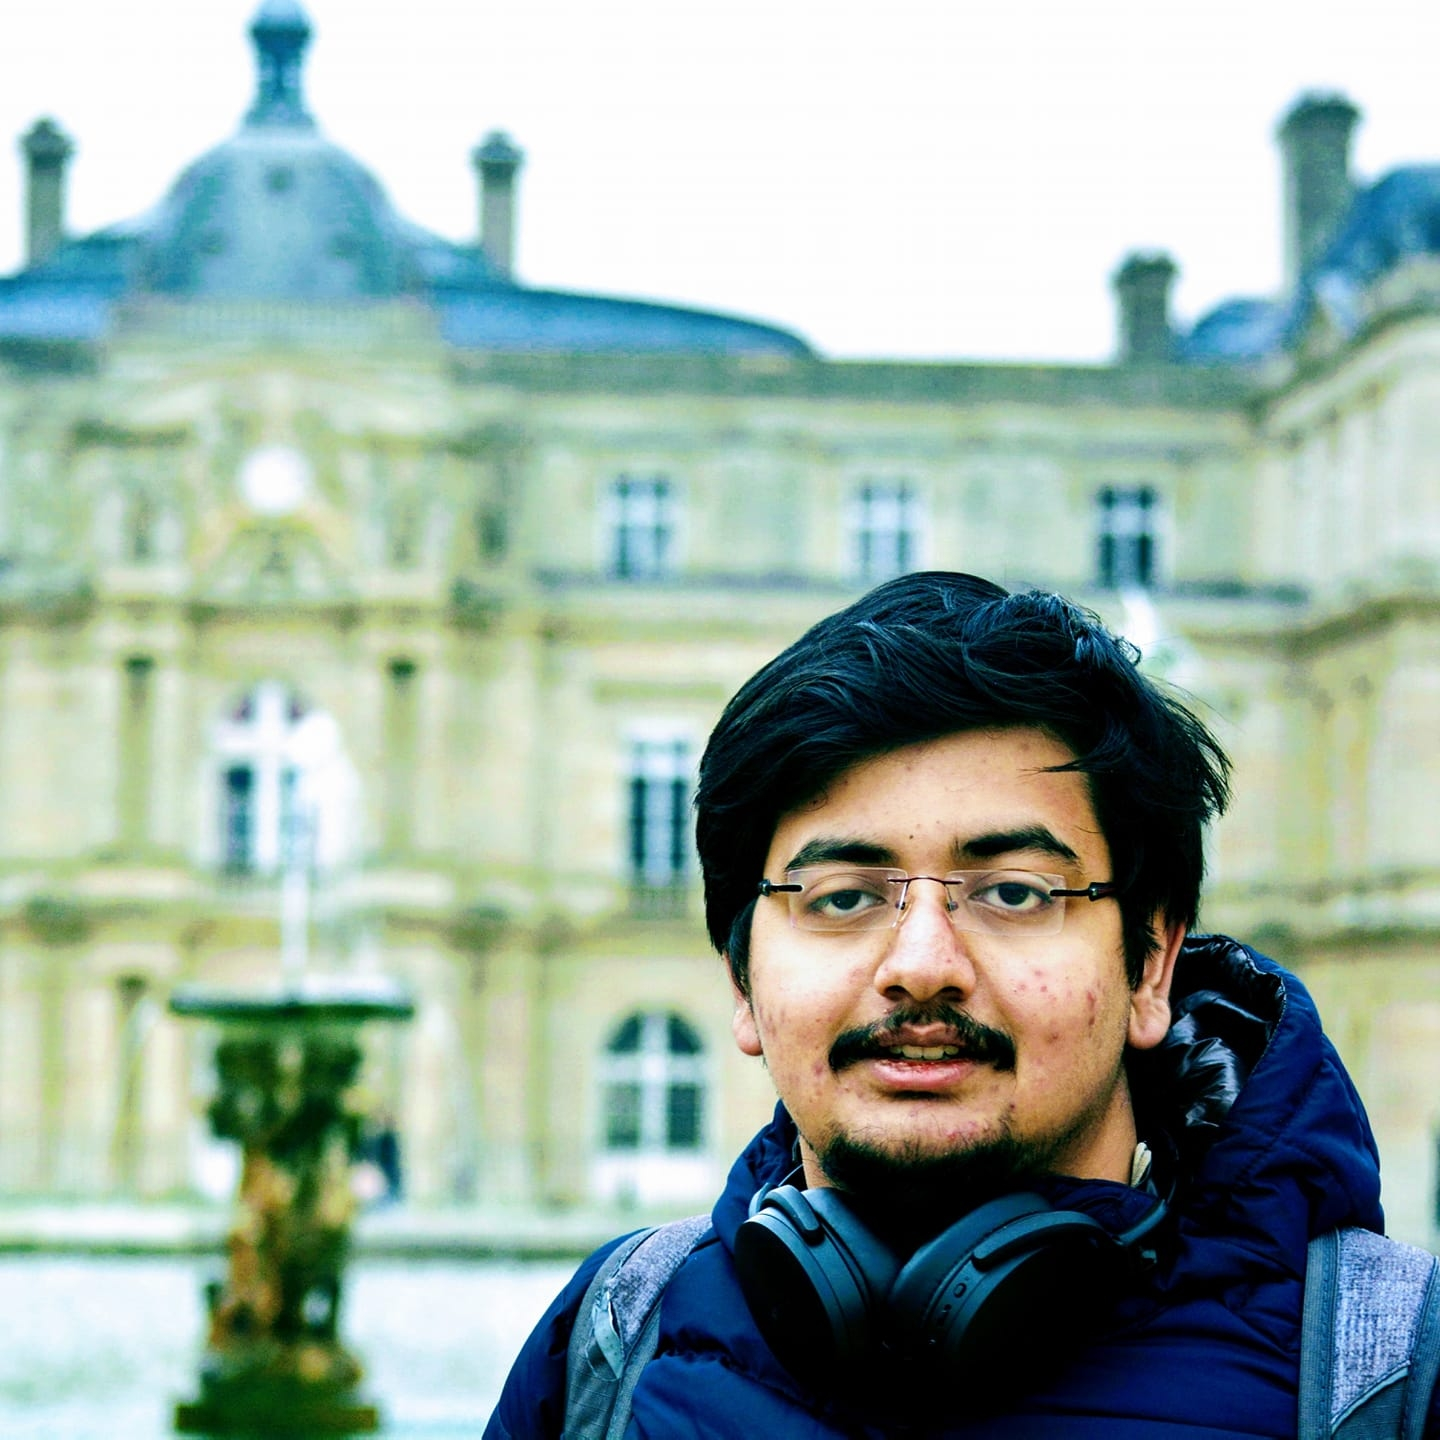
\includegraphics[width=3cm]{self.jpg}}}

\section{Personal Data}
\begin{tabular}{rl}
    \textsc{Place and Date of Birth:} & Kolkata,West Bengal,India  | 04 July 1996 \\
    \textsc{Address:} &  University of Antwerp, Campus Middelheim, Belgium\\
                      %&  M.G.028, 2020 Antwerpen\\
                      %&  België \\
    %\textsc{Phone:}     & +32 465457715 | +917003857712\\
    \textsc{email:}     & \href{mailto:ritam.raha18@gmail.com}{ritam.raha18@gmail.com} | \href{mailto:ritam.raha@uantwerpen.be}{ritam.raha@uantwerpen.be}\\
    \textsc{Current Education:}     & Joint Doctoral Student (cotutelle) in Computer Science\\
    & \href{https://www.uantwerpen.be/en/}{University of Antwerp} \& \href{https://www.labri.fr/}{LaBRI, University of Bordeaux}
\end{tabular}

\section{Research Interest}

My research interest lies in the intersection of \emph{Modelling, Learning \& Verification}. I am interested in learning human-interpretable models from complex systems or modelling them into formal models like Automata, Games and then applying different Formal Verification techniques to ensure safety. My area of interest includes Formal Verification, Logic and Automata, and Artificial Intelligence.


\section{Education}
\begin{tabular}{r|p{11cm}}
\emph{Current} & \\\textsc 2019-Present& \textbf{University of Antwerp, Belgium \& University of Bordeaux, France}\\
& Ph.D. Student in Computer Science\\ 
& Advisor: Guillermo A. P\'erez \& Nathana\"el Fijalkow\\
& \textbf{Research Interest: Formal Methods and Verification, Artificial Intelligence, Logic and Automata Theory, Games}\\&\\
\textsc 2017-2019& \textbf{Chennai Mathematical Institute, India}\\
& M.Sc. in Computer Science
%| CGPA: 9.89
\\
& Advisor: Nicolas Markey \& Loïc Hélouët\\
& \href{https://ritamraha.github.io/thesis/raha_thesis.pdf}{Thesis Title:} Reachability Games With Strong AND Relaxed Energy Constraints\\&\\
\textsc 2014-2017& \textbf{Chennai Mathematical Institute, India}\\
& B.Sc. in Mathematics \& Computer Science
%\\& Computer Science CGPA: 8.13  |  OVERALL CGPA: 7.39 
\\&\\
%\textsc 2012-2014& \textbf{Hindu School}\\
%& Passed 12$^{th}$ standard Board Exam(West Bengal Board of Higher Secondary Education)\\
%& Marks: 448/500 
%\\&\\
%\textsc 2002-2012& \textbf{Baranagore Ramakrishna Mission Ashrama High School}\\
%& Passed 10$^{th}$ standard Board Exam(West Bengal Board of Secondary Education)\\
%& Marks: 633/700 
%\\&\\
\end{tabular}


\section{Publication}
\begin{itemize}
    \item \textsc{(Conference)}
    \href{https://dblp.org/rec/journals/corr/abs-2110-06726}{Scalable Anytime Algorithms for Learning Fragments of Linear Temporal Logic.} TACAS 2022\\
    Ritam Raha, Rajarshi Roy, Nathana\"el Fijalkow, Daniel Neider\\
    \\
    \emph{Description:} Linear temporal logic (LTL) is a specification language for finite sequences (called traces) widely used in program verification, motion planning in robotics, process mining, and many other areas. We consider the problem of learning LTL formulas for classifying traces; In this work, we introduce a new algorithm to this problem which is scalable than existing techniques both in terms of sample size and formula size.
    
    \item \textsc{(Conference)} \href{https://arxiv.org/abs/2005.01071}{Revisiting Parameter Synthesis for One-Counter Automata.} CSL 2022\\
    Guillermo A. P\'erez, Ritam Raha\\
    \\
    \emph{Description:} Our interest in one-counter automata (OCA) with parameters stems from their usefulness as modelling and verifying the behaviour of programs whose control flow is determined by counter variables. We study the synthesis problems for this model that asks, whether there exists a valuation of the parameters such that all infinite runs of the automaton satisfy some $\omega$-regular property. We show that these problems are decidable via reducing it to a newly introduced fragment of Logic.
    
    \item \textsc{(Journal)} \href{https://www.sciencedirect.com/science/article/abs/pii/S089054012100122X}{Reachability Games with Relaxed Energy Constraints.} Information and Computation \\
    Guillermo A. P\'erez, Ritam Raha\\
    \\
    \emph{Description:} This is the extended version of the GandALF paper where we also solves the existence of relaxed bound questions for the Reachability Games.
    
    
    \item \textsc{(Conference)} \href{https://dblp.org/rec/html/journals/corr/abs-1909-07653}{Reachability Games with Relaxed Energy Constraints.} GandALF 2019\\
    Loïc Hélouët, Nicolas Markey, Ritam Raha\\
    \\
    \emph{Description:} Weighted games are a common way to formally address questions related
    to consumption, production and storage of resources. It is a turn-based two player games used in modelling the interactions of the system with its hostile environment. In this work, we solve these games with relaxed upper and lower-bound constraints on the source.
\end{itemize} 


\section{Tool}
- \textsc{SCARLET} (SCalable Anytime algoRithm for LEarning lTl):  A prototype for Learning LTL formulas from positive and negative traces, implemented in Python 3. It is publicly available at \href{https://github.com/rajarshi008/Scarlet}{GitHub}.
 %\pagebreak
\section{Courseworks}
\begin{longtable}{r|p{11cm}}

% \textsc Basic CS Courses&  Automata Theory, Design of Algorithms, Haskel, Python, Java, Data Mining-Machine learning, Model Checking \& System Verification, Complexity Theory, Applied Machine Learning, Logic - Automata \& Games,  Mathematical Logic, Games on Graphs \& Optimization Techniques\\&\\

% \textsc Advanced CS Courses&  Advanced Machine Learning, Concurrent Programming, Linear Programming and Convex Optimization, Games on Graphs 2, Program Analysis, Infinite State Systems, Topics in Security \& Advanced Machine Learning, Logic II, Advanced Algorithms \& Some notions of B \& S automata and Cost Functions(not a formal course), Algebraic Automata Theory,Timed \& Quantitative Automata Theory\\&\\

% \textsc Mathematics Courses&  Algebra I, II \& III (Group, Rings, Vector Spaces, Fields), Calculus I, II \& III, Topology, Differential Equations, Real \& Complex Analysis\\&\\
% \end{longtable}



\textsc CS Courses&  Basic \& Advanced Automata Theory, Design of Algorithms, Data Mining \& Machine learning, Reinforcement Learning, Model Checking \& System Verification, Complexity Theory, Logic - Automata \& Games,   Optimization Techniques, Concurrent Programming, Linear Programming and Convex Optimization \\&\\

\textsc Programming Courses& Python, Java, Haskell, Applied Machine Learning\\&\\

\textsc Mathematics Courses&  Algebra I, II \& III (Group, Rings, Vector Spaces, Fields), Calculus I, II \& III, Topology, Differential Equations, Real \& Complex Analysis\\&\\
\end{longtable}




%Master's Thesis on Quantitative Reachability Games with Nicolas Markey %and Loic Helouet in INRIA Rennes\\&\\
 
%\textsc M.Sc. 2$^{nd}$ semester&  Computer Science Courses : Games on %Graphs 2, Program Analysis, Model Checking \& System Verification\\&\\

%
%\textsc M.Sc. 1$^{st}$ semester&  Computer Science Courses : Data Mining-Machine learning, Infinite State Systems, Topics in Security \& Advanced Machine Learning\\&\\

% \textsc B.Sc. 6$^{th}$ semester& Computer Science Courses : Concurrency Theory, Logic II, Advanced Algorithms \& Some notions of B \& S automata and Cost Functions(not a formal course)\\&\\

%\textsc B.Sc. 5$^{th}$ semester& Computer Science Courses : Logic - Automata \& Games, Algebraic Automata Theory, Mathematical Logic, Games on Graphs \& Optimization Techniques\\&\\

%\textsc B.Sc. 4$^{th}$ semester& Computer Science Courses : Programming Language Concepts(Java,$ \lambda$-Calculus) \& Quantitative Automata Theory(Sequential Transducers, Weighted Automata \& Timed Automata)  \\
%& Math Courses : Topology, Differential Equations, Complex Analysis\\&\\

%\textsc B.Sc. 3$^{rd}$ semester& Computer Science Courses : Design and Analysis of Algorithms \& Theory of Computation\\
%& Math Courses : Algebra III, Real Analysis, Calculus III\\&\\

%\textsc B.Sc. 2$^{nd}$ semester& Computer Science Courses : Advanced Programming(Python), Discrete Math\\
%& Math Courses : Algebra II, Calculus II, Probability Theory\\&\\

%\textsc B.Sc. 1$^{st}$ semester& Computer Science Courses :  Introduction to Haskell\\
%& Math Courses : Algebra I, Calculus I\\&\\
%\end{longtable}





\section{Internship Experience}
\begin{longtable}{r|p{11cm}}

\textsc {Winter 2018} & \textbf {Master's Intern at INRIA, Rennes}\\
& Worked under Prof. Nicolas Markey and Prof. Loic Helouet  on "Reachability Games with Relaxed Energy Constraints"\\&\\


\textsc {Summer 2018} & \textbf {Research Intern at LaBRI, Bordeaux}\\
& Worked under Prof. Nathanael Fijalkow, Vincent Penelle, Filip Mazowiecki and Nathan Lhote  on "Weighted Automata with Ambiguity and Extensions"\\&\\

\textsc {Summer 2017} & \textbf {Research Intern at LSV, ENS Cachan}\\
& Worked under Prof. Philippe Schnoebelen  on "Piecewise Testable Index of Words
and Its Algorithmic Evaluation"\\&\\

 \textsc {Summer 2016} & \textbf {Summer Intern at Institute of Mathematical Sciences, Chennai}\\
& Worked under Prof. Teodor Knapik, a visiting faculty at IMSc., from University of Caledonia, on "\emph{Automatic Structures and Presentations}" and also an official intern at TCS summer programme by IMSc.\\&\\

% \textsc {Summer 2015} & \textbf {Summer Intern at Indian Statistical Institute, Kolkata}\\
% & Worked under Prof. Sandip Das and Prof. Sagnik Sen on "\emph{Some approach to Borodin-Kostochka Conjecture}" \\
\end{longtable}

\section{Research Experience \& Talks}
\begin{itemize}
    \item Reviewed several papers in peer-reviewed conferences and journals e.g., FORMATS, FSTTCS, IC, IPL
    
    \item Presented my work in several workshops and conferences like HIGHLIGHTS \& MOVEP 
    
    \item Presented my work in weekly seminars in different universities
    
    %\item Piecewise Testable Index of Words and Its Algorithmic Evaluation, Student Symposium on Verification, Automata and Games, Chennai Mathematical Institute, India
    
    %\item Automatic Structure and First order Decidability, Institute of Mathematical Sciences
\end{itemize}
\section{Teaching Experience}
\begin{itemize}
\item Co-supervised Master's Thesis Internship for two Computer Science students in the University of Antwerp
\item Worked as a Teaching-Assistant on "Concurrency Theory" course under Prof. Madhavan Mukund
\item Worked as a Teaching-Assistant on "Mathematical Logic" course under Prof. M. Praveen
\item Worked as a part-time teacher for VISTAMIND, Chennai
\end{itemize}

\section{Scholarships and Certificates}
\begin{tabular}{rl}
 \textsc {October} 2019 & Recipient of Doctoral Scholarship Programme of University of Antwerp\\
 
 \textsc {December} 2018 & Selected winner in Poster Competition organised by \textit{Tata Consultancy Services}\\ &for presenting "Synthesis via Multi-Criteria Quantitative Games".\\
 
 %\textsc{AUG} 2017 & Recipient of Chennai Mathematical Institute Master's Scholarship\\
 
 \textsc{FEB} 2016 & Recipient of \href{http://www.online-inspire.gov.in/}{INSPIRE} scholarship programme\\
\end{tabular}




\section{Programming Skills}
\begin{tabular}{rl}
 Basic Knowledge:& Haskell, Java, \textsc{html \& CSS}, C++\\
Advanced Knowledge:&  Python, {\fb \LaTeX}\setmainfont[SmallCapsFont=Fontin-SmallCaps.otf]{Fontin.otf}\\
\end{tabular}

\section{Extra-curricular}
\begin{itemize}
\item Loves to play Ukulele
 \item Interested in sports (mainly Football)
 \item Loves recitation and participated at many cultural programmes in school and college
\end{itemize}



\section{References}
\begin{itemize}
\item {\href{https://www.uantwerpen.be/en/staff/guillermoalberto-perez/}{\textbf {Guillermo Alberto Perez}}}\ \ {\textit {Head of the Formal Techniques in Software Engineering (FOTS) lab, a part of the AnSyMo research group.}}
 \begin{description}
  Email Id: 	guillermoalberto.perez@uantwerpen.be  
  \end{description}

\item {\href{https://nathanael-fijalkow.github.io/}{\textbf {Nathanael Fijalkow}}}\ \ {\textit {full-time (permanent) researcher at CNRS in LaBRI, Bordeaux}}
 \begin{description}
  Email Id: nathanael.fijalkow@labri.fr 
  \end{description}

\item {\href{http://people.irisa.fr/Nicolas.Markey/}{\textbf {Nicolas Markey}}}\ \ {\textit {CNRS senior researcher at IRISA}}
 \begin{description}
  Email Id: 	nicolas.markey@irisa.fr  
  \end{description}
  
  \item {\href{https://www.cmi.ac.in/~sri/}{\textbf {B. Srivathsan}}}\ \ {\textit {Professor, Chennai Mathematical Institute}}
 \begin{description}
  Email Id: sri@cmi.ac.in
  \end{description}
 
 \item {\href{http://www.cmi.ac.in/~madhavan/}{\textbf {Madhavan Mukund}}}\ \ {\textit {Professor and Dean of Studies, Chennai Mathematical Institute}}
 \begin{description}
  Email Id: madhavan@cmi.ac.in
  \end{description}
 
\end{itemize}

\end{document}
